\documentclass{article}
\usepackage{graphicx} % Required for inserting images
\usepackage{subcaption}


\author{Simone La Bella}
\date{May 2024}

\begin{document}


\section{Omografia e calcolo prospettiva}
Una parte fondamentale del progetto è stata la calibrazione della camera, in particolare era importante capire o simulare il grandangolo e il fuoco della lente. L'obiettivo finale era quello di mappare le posizioni all'interno dell'immagine data in input, con la posizione relativa in un campo da calcio 2D, tramite una \textbf{matrice di omografia} [link wikipedia]. 
Questo passaggio è fondamentale ai fini della riuscita del progetto, per rendere più veloce il calcolo del fuorigioco e per dare piu informazioni all'utente. Sono state percorse varie idee, prima di arrivare alla soluzione finale.
\\
\subsection{Approci sperimentali}
La prima è stata quella di effettuare una maschera sul campo tramite OpenCV, in modo da eliminare gli spalti per avere meno informazioni superflue possibili, che avrebbero potuto alterare il risultato. [Fig 1]  

\begin{figure}[h]
    \centering
    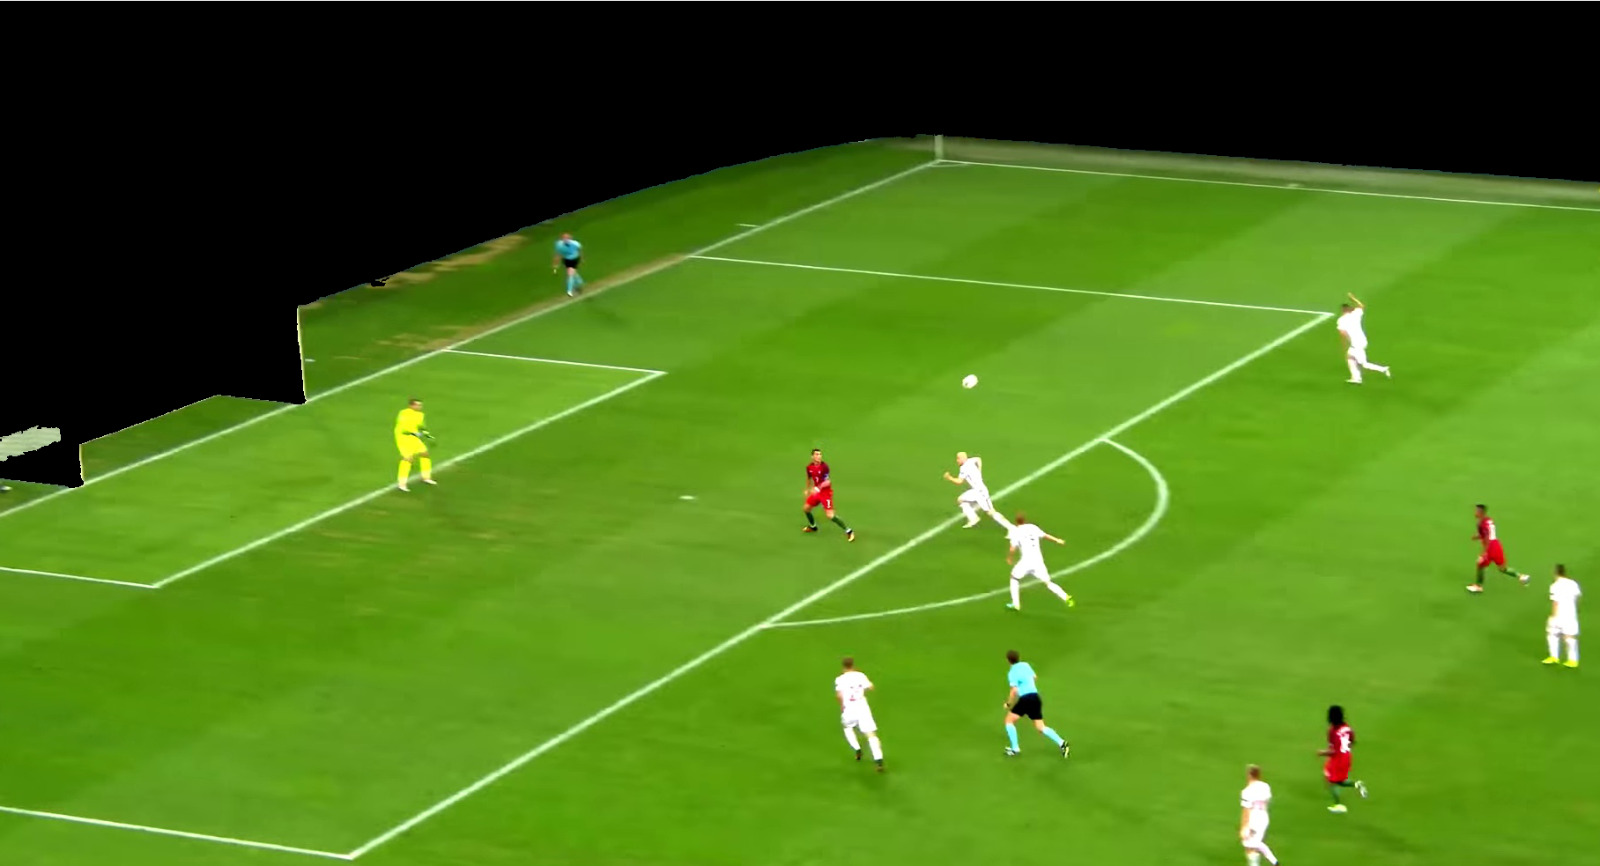
\includegraphics[width=0.7\linewidth]{capitoli/senzaSpalti.jpg}
    \caption{Immagine risultante dopo l'eliminazione degl spalti tramite maschere e operazioni bitwise}
    \label{fig:enter-label}
\end{figure}

In seguito alla maschera sono state effettuate delle operazioni sull'immagine in modo da pre-processarla [Fig 2a], per migliorare la possibilità di individuare le linee del campo tramite la funzione \textbf{RoughLinesP()} [link documentazione OpenCV], per individuare 4 punti, non su una stessa linea, che ci avrebbero permesso di calcolare la matrice di omografia dell'immagine, in modo da poter mappare i punti su un immagine 2D. Il problema di questo metodo si riscontra nella radice del nostro progetto, ovvero le immagini del campo, che essendo di una qualità non elevata, rendevano impossibile per la funzione individuare in maniera netta le linee, anche se ad occhio umano sarebbero potute sembrare ben delineate. [Fig 2b] 

\begin{figure}[h]
    \centering
    \begin{subfigure}{0.33\textwidth}
        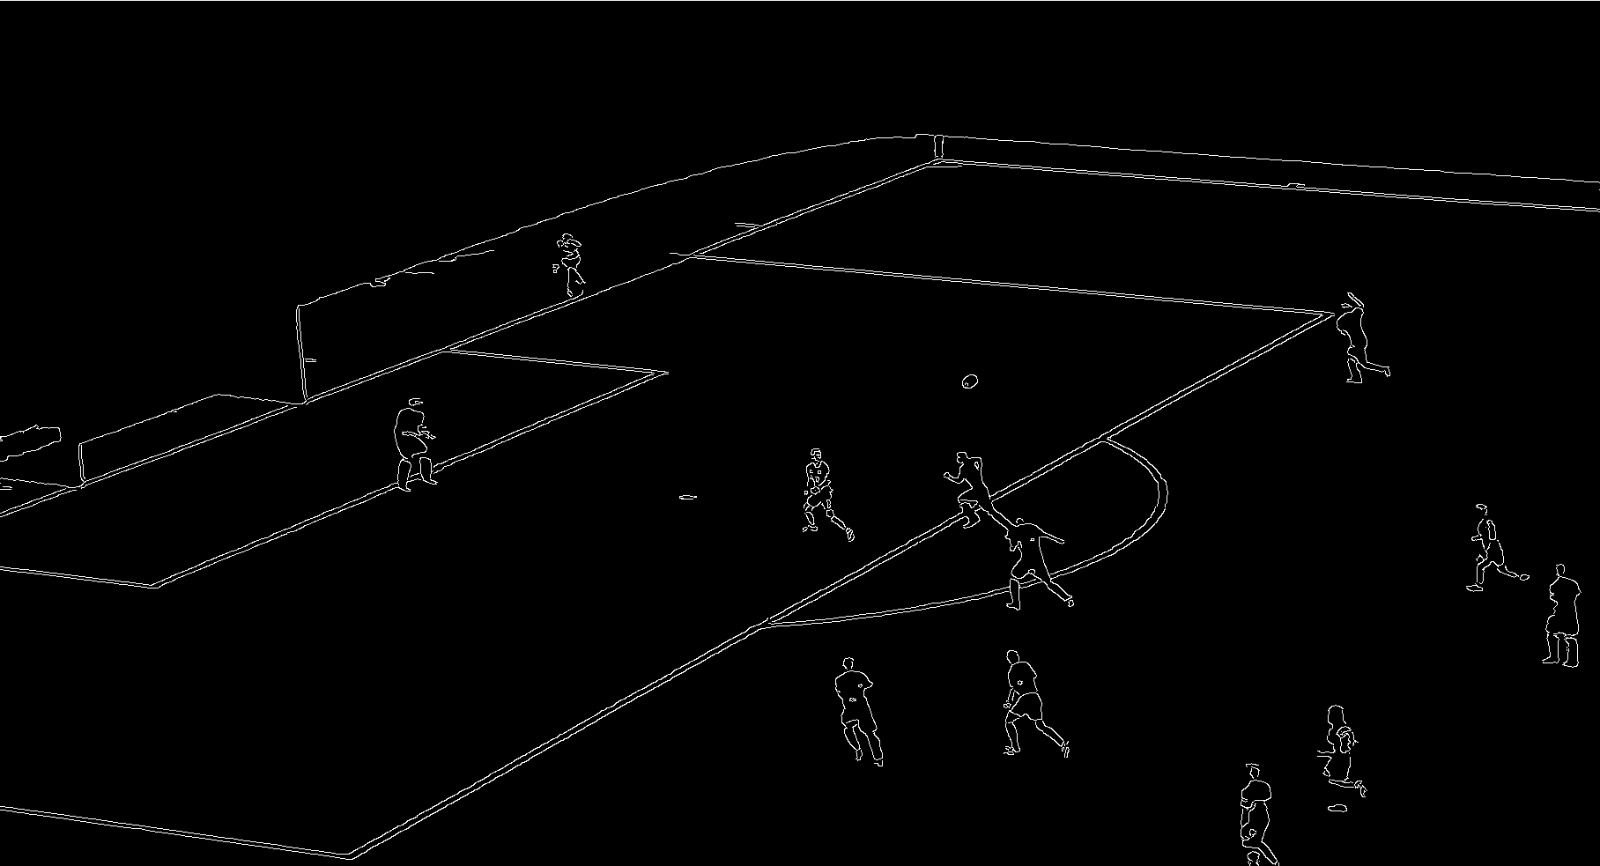
\includegraphics[width=\linewidth]{capitoli/cannyimage.jpeg}
        \subcaption{}
    \end{subfigure}
    \begin{subfigure}{0.40\textwidth}
        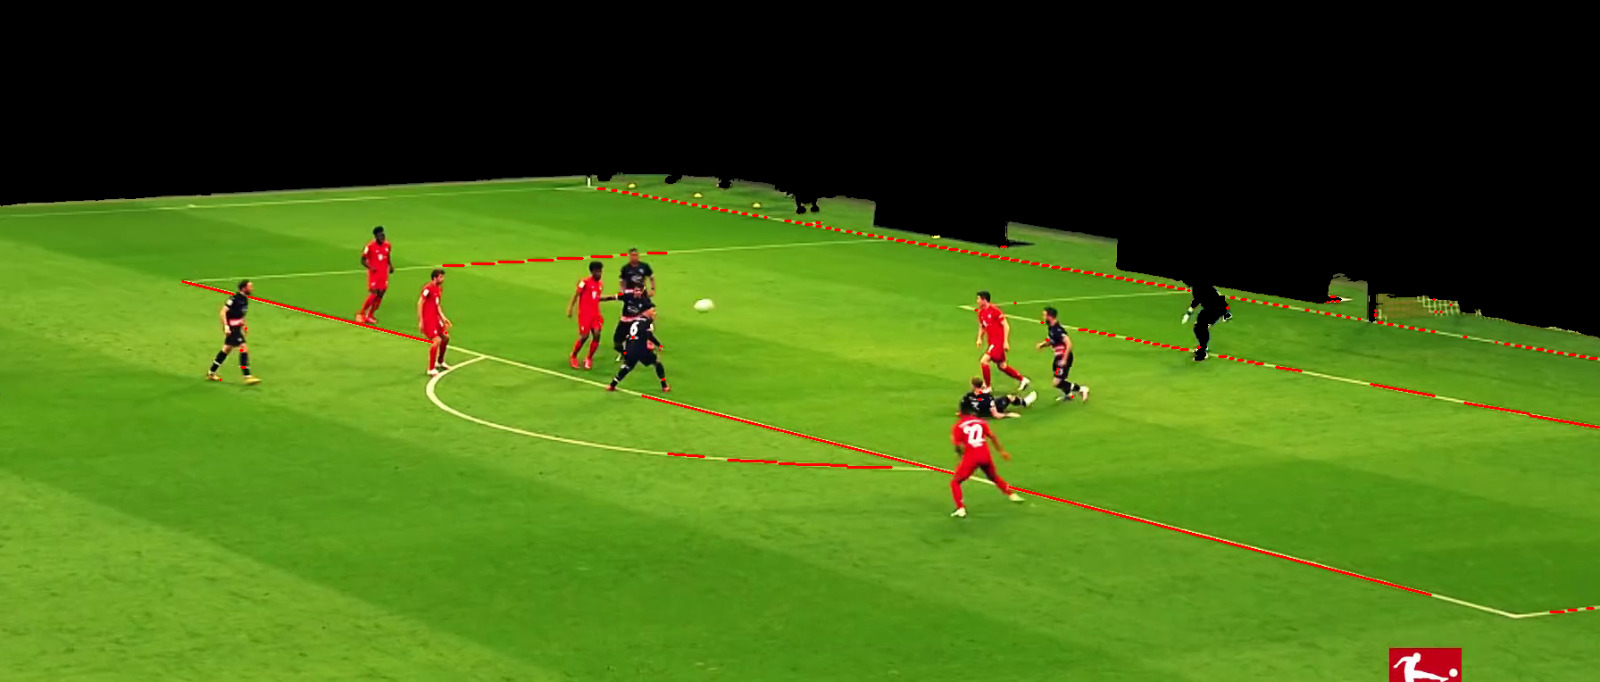
\includegraphics[width=\linewidth]{capitoli/roughlines.jpeg}
        \subcaption{}
    \end{subfigure}
    \caption{a: Immagine processata per facilitare l'individuamento delle linee maschere, b: Immagine risultante dopo aver applicato RoughLinesP}
    \label{fig:foobar}
\end{figure}

A seguito di questi problemi, è stato deciso di provare ad utilizzare un altro approccio, ovvero una soluzione che sfruttasse il \textbf{punto di fuoco} dell'immagine rispetto alla prospettiva, per alcuni punti fondamentali all'interno del campo, cosi da permetterci di effettuare una proiezione. 
In particolare, la soluzione da noi proposta cercava di tracciare delle linee nel campo in modo tale che fossero parallele o conformi alle linee del campo da calcio all'interno dell'immagine. Dopo aver individuato 2 linee principali, venivano prolungate fino a che non si fosse riscontrata un intersezione fra le due linee, ovvero il punto di fuoco.

\begin{figure}[h]
    \centering
    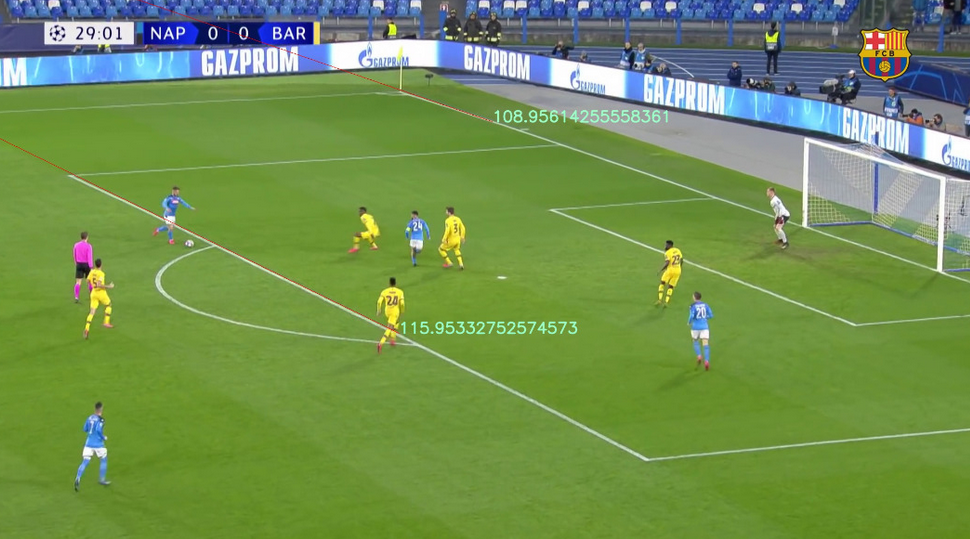
\includegraphics[width=0.7\linewidth]{capitoli/vanishingpoint.png}
    \caption{Immagine risultante dopo aver individuato il punto di fuoco, i numeri in verde sono i gradi della linea}
    \label{fig:enter-label}
\end{figure}

Anche questa metodologia riscontrava delle gravi problematiche, per immagini con prospettive molto orizzontali rispetto al campo, ovvero quando il punto di fuoco era presente all'interno dell'immagine, non era possibile individuare delle linee in modo corretto, ed inoltre non era possibile effettuare una proiezione 2D dei punti all'interno dell'immagine, essendo che le linee individuate erano in una posizione casuale dell'immagine. Quindi se avessimo dovuto solamente individuare il fuorigioco, la seguente metodologia avrebbe funzionato, però ai fini del nostro progetto era anche molto importante poter avere una rappresentazione 2D del campo e dei giocatori. Per questi motivi, è stato deciso di scartare anche questa opzione.
\\
\\

\subsection{Approccio finale}
Il metodo migliore che abbiamo trovato è stato l'utilizzo di un modello di Deep Learning [Bibliografia], che ci ha permesso di individuare la prospettiva corretta e di calcolare la matrice di omografia dell'immagine. Abbiamo dovuto adattare il modello per farlo lavorare su singoli frame, essendo stato creato per lavorare sui video.
\\ \\
Il modello in particolare ha come obiettivo l'utilizzo del Deep Learning [link wikipedia] per effettuare una regressione sugli errori, in modo da trovare i parametri di registrazione che minimizzano l'errore. Nello specifico propone una pipeline di reti neurali, che vengono utilizzate in modo sequenziale e ciclico. 
\\La prima rete neurale è chiamata \textit{Initial registration network}, permette di ottenere una stima dei parametri di registrazione e della corrispettiva matrice di omografia, fornendo in input alla rete neurale seguente, l'immagine presa in input e l'immagine di un campo 2D inserito in prospettiva tramite un warping nell'immagine in input, sfruttando i parametri e l'omografia ottenuti. 
\\La seconda rete neurale, viene chiamata \textit{Registration network error} e si occupa di minimizzare l'errore stimato dalla precedente rete, tramite una regressione. Nello specifico prende in ingresso i dati dalla rete neurale precedente, stima l'errore dell'omografia in base all'immagine presa come input, e tramite differenziazione e backpropagation, viene individuata la direzione nella quale l'errore viene minimizzato. La seguente operazione viene ripetuta iterativamente finché non viene raggiunto un obiettivo o non vengono raggiunte un numero prestabilito di operazioni.

\begin{figure}[h]
    \centering
    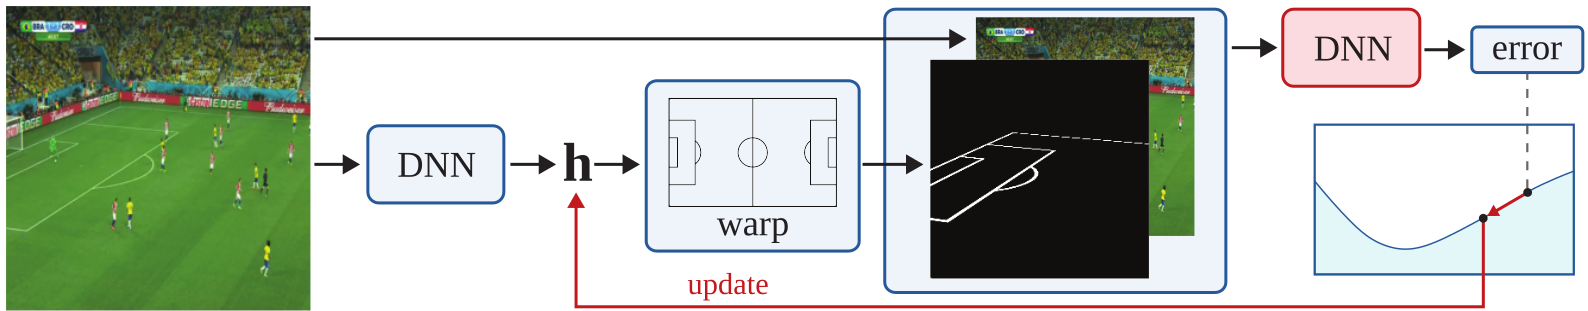
\includegraphics[width=1\linewidth]{capitoli/reteNeurale.png}
    \caption{Illustrazione del modello}
    \label{fig:enter-label}
\end{figure}

Possiamo quindi affermare in breve, che la prima rete neurale si occupa di fornire una stima approssimativa e non accurata della prospettiva e dell'omografia, ed in seguito, la seconda rete neurale si occupa di ottimizzare al massimo i parametri ottenuti, utilizzando un metodo che gli autori chiamano \textit{inference through optimization}, che permette di essere significativamente più accurati rispetto ai modelli classici che utilizzano il metodo del \textit{forwarding}.

Nello specifico, il metodo \textit{inference through optimization}, ha come scopo insegnare ad un modello a decretare quanto bene due immagini sono allineate. 
\\Il modello, a quanto affermato, è lo \textit{state-of-the-art} rispetto al dominio \textit{Camera calibration}, fornendo una stima molto accurata della prospettiva, gli autori affermano inoltre che il loro metodo di creazione del modello, è il primo che permette di imparare a regredire gli errori a partire da un immagine già ottimizzata.
\\\\
Un progetto affine al modello precedentemente descritto è il \textit{deep value network}, dove una rete neurale viene allenata per stimare la sezione di intersezione rispetto a due unioni, ovvero la stima del parametro \textit{IoU}.
\\È stato provato l'utilizzo di questo metodo, pero non ha fornito i risultati attesti e difatti, nel paper, gli autori esprimono il proprio giudizio riguardante il modello deep value network, in quanto esso, richiede una lunga ottimizzazione della traiettoria ed è inoltre limitato ad una sola iterazione iniziale, senza possibilità di miglioramenti.

\subsubsection{Dettagli pratici}

Per ottenere un omografia valida, è fondamentale avere un minimo di 4 punti non su una stessa linea. Il modello, come precedentemente descritto, crea una matrice di omografia fra l'immagine di gioco e il campo 2D, prendendo 4 punti che tipicamente contengono la visuale del campo dal basso, i punti sono descritti con i seguenti valori:
\begin{itemize}
    \item(-0.5, 0.1): angolo inferiore sinistro del rettangolo
    \item(-0.5, 0.5): angolo superiore sinistro del rettangolo
    \item(0.5, 0.5): angolo superiore destro del rettangolo
    \item(0.5, 0.1): angolo inferiore destro del rettangolo
\end{itemize}
\begin{figure}[h]
    \centering
    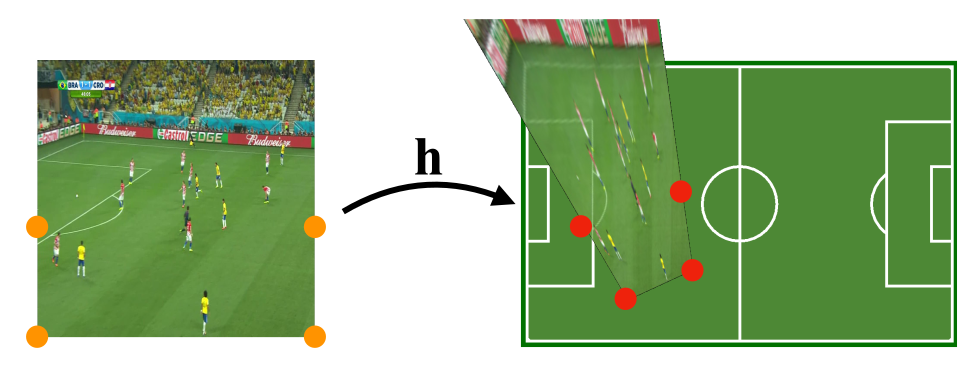
\includegraphics[width=0.7\linewidth]{capitoli/Hiniziale.png}
    \caption{Illustrazione dei punti di controllo per generare la matrice di omografia}
    \label{fig:enter-label}
\end{figure}
Andando a formare un lista \textbf{\begin{math}{h_{ref}}\end{math}} dove \begin{math}{u_1, v_1}\end{math} indicano la x e la y di un punto:
\[ \textbf{{\begin{math}{h_{ref}}\end{math}}} = [u_1, v_1, u_2, v_2, u_3, v_3, u_4, v_4 ] \]

Utilizzando i punti stimati in \textbf{{\begin{math}{h_{ref}}\end{math}}} e l'algoritmo di ottimizzazione \textbf{Adam}, è possibile ottenere una convergenza stabile durante l'ottimizzazione e quindi una matrice di omografia.
In particolare l'algoritmo Adam [Citazione al sito arxviv su algoritmo adam] permette di ottenere un ottimizzazione basata sul gradiente di primo ordine di una funzione. Questo algoritmo permette di addestrare modello di reti neurali, combinando i vantaggi di AdaGraf e RMSProp, adattando il learning rate per ciascun hyper-parameter. 
\\\\
I dataset utilizzati per validare ed addestrare il modello sono due.
Il primo è 'The World Cap dataset'[Link prendere dal paper], composto da 395 immagini divise fra training, validation e testing. Il secondo dataset è utilizzato riguarda la corrispondenza fra  il campo da calcio nell'immagine ed il template 2D, sono state utilizzate 39 immagini divise come per il precedente dataset fra training, validation e testing. 
I dati sono stati trattati con la tecnica del \textit{Data augmentation} per aumentare i sample e per migliorare il funzionamento del modello proponendo scenari e casistiche differenti.
\\\\
Entambi i modelli si basano su un architettura molto conosciuta, ovvero ResNet-18, opportunamente modificata dagli autori.
\begin{figure}[h]
    \centering
    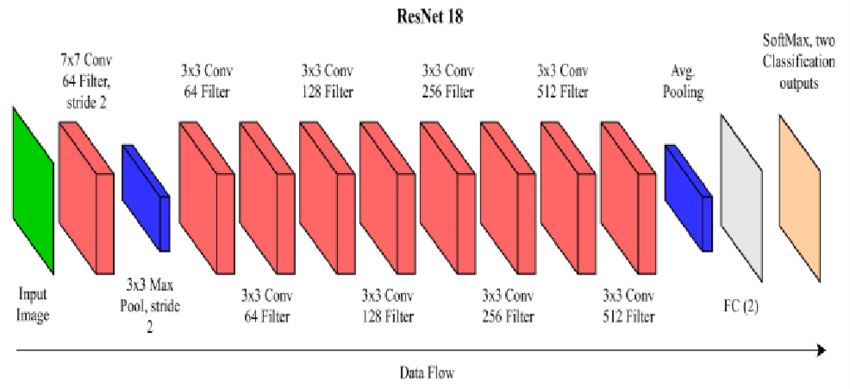
\includegraphics[width=0.7\linewidth]{capitoli/resnetArch.png}
    \caption{Illustrazione dell'architettura}
    \label{fig:enter-label}
\end{figure}

Nel primo modello, è stata sostituita la parte finale, ovvero la testa, con un ultimo layer nella quale convergono tutti i nodi della rete (fully connected layer), utilizzato per stimare gli 8 numeri che vanno poi a rappresentare l'omografia.
Nel secondo modello su tutti i livelli è stata applicata una spectral normalization, ovvero una tecnica di normalizzazione utilizzata per stabilizzare l'allenamento del discriminante [link paperwithcode].
Sull'ultimo livello (head) è stata applicata una funzione \textit{sigmoid} per rendere il risultato positivo, ed una funzione per la riproiezione dell'errore metrico.

\subsubsection{Risultati}

I risultati del modello sono eccellenti, come si può evincere dal risultato [Fig 7], l'ottimizzazione è un fattore chiave per la precisione finale, dovendo effettuare un training personalizzato su ogni immagine che viene inserita in input, rendendo cosi la velocità del modello dipendente dall'hardware della macchina. 


\begin{figure}[h]
    \centering
    \begin{subfigure}{0.45\textwidth}
        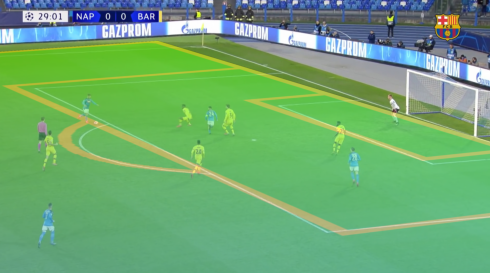
\includegraphics[width=\linewidth]{capitoli/HpitchSample.png}
        \subcaption{}
    \end{subfigure}
    \begin{subfigure}{0.45\textwidth}
        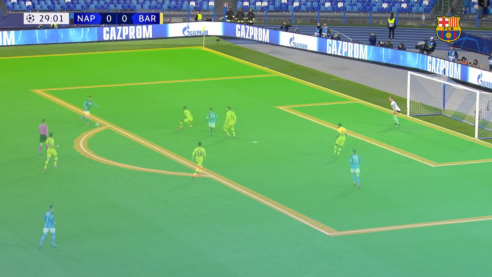
\includegraphics[width=\linewidth]{capitoli/HpitchOptimSample.png}
        \subcaption{}
    \end{subfigure}
    \caption{a: Immagine iniziale derivante dal primo modello, b: Immagine risultante dopo l'ottimizzazione tramite 200 iterazioni}
    \label{fig:foobar}
\end{figure}

 Un miglioramento che si potrebbe attuare al modello sarebbe la sostituzione della seconda parte, l'ottimizzazione, che rende tutto il processo di lavorazione dell'immagine molto lento, a favore di un miglioramento del primo modello, tramite per esempio un cambio architettura alla base. 
\\\\
 In conclusione, il modello ci ha permesso di ottenere i dati che servivano al progetto, ovvero la matrice di omografia, per effettuare una corrispondenza quanto più precisa possibile dei punti in 3D su un template 2D.

\end{document}